
% 1. Стиль и язык
\documentclass[utf8x]{G7-32} % Стиль (по умолчанию будет 14pt)
\usepackage[T2A]{fontenc}
\usepackage[russian]{babel}

% Псевдокод
\usepackage[]{algorithm2e}
\newenvironment{rualgorithm}[1][htb]
  {\renewcommand{\algorithmcfname}{Алгоритм}% Update algorithm name
   \begin{algorithm}[#1]%
  }{\end{algorithm}}

% Фикс отступа в оглавлении
\makeatletter
\renewcommand*\l@subsection{\@dottedtocline{1}{2em}{3.0em}}
\makeatother

% Остальные стандартные настройки убраны в preamble.inc.tex.
\sloppy

% Настройки стиля ГОСТ 7-32
% Для начала определяем, хотим мы или нет, чтобы рисунки и таблицы нумеровались в пределах раздела, или нам нужна сквозная нумерация.
\EqInChapter % формулы будут нумероваться в пределах раздела
\TableInChapter % таблицы будут нумероваться в пределах раздела
\PicInChapter % рисунки будут нумероваться в пределах раздела

% Добавляем гипертекстовое оглавление в PDF
\usepackage[
bookmarks=true, colorlinks=true, unicode=true,
urlcolor=black,linkcolor=black, anchorcolor=black,
citecolor=black, menucolor=black, filecolor=black,
]{hyperref}

% Изменение начертания шрифта --- после чего выглядит таймсоподобно.
% apt-get install scalable-cyrfonts-tex

\IfFileExists{cyrtimes.sty}
    {
        \usepackage{cyrtimespatched}
    }
    {
        % А если Times нету, то будет CM...
    }

\usepackage{graphicx}   % Пакет для включения рисунков

% С такими оно полями оно работает по-умолчанию:
% \RequirePackage[left=20mm,right=10mm,top=20mm,bottom=20mm,headsep=0pt]{geometry}
% Если вас тошнит от поля в 10мм --- увеличивайте до 20-ти, ну и про переплёт не забывайте:
\geometry{right=20mm}
\geometry{left=30mm}


% Пакет Tikz
\usepackage{tikz}
\usetikzlibrary{arrows,positioning,shadows}

% Произвольная нумерация списков.
\usepackage{enumerate}

% ячейки в несколько строчек
\usepackage{multirow}

% itemize внутри tabular
\usepackage{paralist,array}


% Настройки листингов.
% 8 Листинги

\usepackage{listings}

% Значения по умолчанию
\lstset{
  basicstyle= \footnotesize,
  breakatwhitespace=true,% разрыв строк только на whitespacce
  breaklines=true,       % переносить длинные строки
%   captionpos=b,          % подписи снизу -- вроде не надо
  inputencoding=koi8-r,
  numbers=left,          % нумерация слева
  numberstyle=\footnotesize,
  showspaces=false,      % показывать пробелы подчеркиваниями -- идиотизм 70-х годов
  showstringspaces=false,
  showtabs=false,        % и табы тоже
  stepnumber=1,
  tabsize=4,              % кому нужны табы по 8 символов?
  frame=single
}

% Стиль для псевдокода: строчки обычно короткие, поэтому размер шрифта побольше
\lstdefinestyle{pseudocode}{
  basicstyle=\small,
  keywordstyle=\color{black}\bfseries\underbar,
  language=Pseudocode,
  numberstyle=\footnotesize,
  commentstyle=\footnotesize\it
}

% Стиль для обычного кода: маленький шрифт
\lstdefinestyle{realcode}{
  basicstyle=\scriptsize,
  numberstyle=\footnotesize
}

% Стиль для коротких кусков обычного кода: средний шрифт
\lstdefinestyle{simplecode}{
  basicstyle=\footnotesize,
  numberstyle=\footnotesize
}

% Стиль для BNF
\lstdefinestyle{grammar}{
  basicstyle=\footnotesize,
  numberstyle=\footnotesize,
  stringstyle=\bfseries\ttfamily,
  language=BNF
}

% Определим свой язык для написания псевдокодов на основе Python
\lstdefinelanguage[]{Pseudocode}[]{Python}{
  morekeywords={each,empty,wait,do},% ключевые слова добавлять сюда
  morecomment=[s]{\{}{\}},% комменты {а-ля Pascal} смотрятся нагляднее
  literate=% а сюда добавлять операторы, которые хотите отображать как мат. символы
    {->}{\ensuremath{$\rightarrow$}~}2%
    {<-}{\ensuremath{$\leftarrow$}~}2%
    {:=}{\ensuremath{$\leftarrow$}~}2%
    {<--}{\ensuremath{$\Longleftarrow$}~}2%
}[keywords,comments]

% Свой язык для задания грамматик в BNF
\lstdefinelanguage[]{BNF}[]{}{
  morekeywords={},
  morecomment=[s]{@}{@},
  morestring=[b]",%
  literate=%
    {->}{\ensuremath{$\rightarrow$}~}2%
    {*}{\ensuremath{$^*$}~}2%
    {+}{\ensuremath{$^+$}~}2%
    {|}{\ensuremath{$|$}~}2%
}[keywords,comments,strings]

\newcommand\pythonstyle{\lstset{
language=Python,
basicstyle=\ttm,
otherkeywords={self},             % Add keywords here
keywordstyle=\ttb\color{deepblue},
emph={MyClass,__init__},          % Custom highlighting
emphstyle=\ttb\color{deepred},    % Custom highlighting style
stringstyle=\color{deepgreen},
frame=tb,                         % Any extra options here
showstringspaces=false            % 
}}

% Подписи к листингам на русском языке.
\renewcommand\lstlistingname{\cyr\CYRL\cyri\cyrs\cyrt\cyri\cyrn\cyrg}
\renewcommand\lstlistlistingname{\cyr\CYRL\cyri\cyrs\cyrt\cyri\cyrn\cyrg\cyri}


% Полезные макросы листингов.
% Любимые команды
\newcommand{\Code}[1]{\textbf{#1}}


% Сквозная нумерация
\usepackage{chngcntr}
\counterwithout{figure}{chapter}
\counterwithout{table}{chapter}


\title{Diploma}
\author{chesterlanduk }
\date{May 2019}

\begin{document}

\frontmatter
\setcounter{page}{2}

% Убрать токи в оглавлении
\makeatletter
\renewcommand{\@dotsep}{10000} 
\makeatother

\tableofcontents


% \maketitle

\Introduction
\chapter{ВВЕДЕНИЕ}


Информатикс -- информационный ресурс (далее -- сайт), расположенный в сети Интернет 
и доступный по доменным адресам \texttt{informatics.msk.ru} и \texttt{informatics.mccme.ru}.

Сайт представляет собой сборник задач по программированию различной сложности, от уровня начинающих и до задач уровня международных олимпиад. 
Задачи можно решать -- прогонять на тестах программный код, который протестируется системой. 
После прохождения тестов пользователю сайта выдается результат тестирования в виде количества пройденных тестов, 
статусе успешности или неуспешности решения задачи, сообщение компилятора или интерпретатора.
Помимо этого, сайт представляет фунцкионал создания курсов и уроков на основе существующих задач.
Также у сайта есть функционал управления обучением (англ. Learnging Management System -- далее по тексту LMS).

Сайт имеет более 300 тысяч пользователь, а месячное количество активных пользователей достигает 40 тысяч человек.

К сожалению, с течением времени функционал сайта становился всё менее стабильным, 
из-за глубинных архитектурных проблем им становилось всё сложнее пользоваться\cite{inf_not_working}.


\mainmatter % это включает нумерацию глав и секций в документе ниже

% \input{0-1-literaly-review.tex}

\chapter{Содержательная постановка задачи}

\section{Описание рабты существующей системы}

С точки зрания архитектуры программного продукта Информатикс делится на следующие части:

\begin{itemize}
    \item Moodle -- в качестве основного web-интерфейса сайта;
    \item Ejudge -- в качестве тестирующей системы;
    \item различные самописные модули на PHP, например, для управления группами учеников и для отрисовки наборов задач (далее по тексту -- конестов);
    \item различные самописные модули и API на Python, предоставляющие доступ к протоколам тестирования, сдачи кода пользователей и другое.
    \item СУБД MySQL 5.5.
\end{itemize}

Рассмотрим каждую часть подробнее.

\subsection{Ejudge}

Ejudge -- система для проведения различных мероприятий, в которых необходима автоматическая проверка программ. 
Она была разработана Алекстандром Черновым, предподавателем МГУ, в 2004 году. 
Система активно доробатывается и на текущий момент имеет более 11 тысяч коммитов в официальном репозитории.
Помимо этого, существует много различных дополнений системы, таких, как, например, 
патч к ядру Linux для более безопасного исполнения кода, ограничивающий доступ программы к некоторым возможностям операционной системы,
или файловая система, построенная на технологии FUSE, предоставляющая интерфейс сдачи задач в виде копирования файла с исходников в определенную примонтированную директорию.

Ejudge поддерживает следующие возиожности:

\begin{itemize}
    \item Проведение турниров с автоматической проверкой задач по четырём системам: ACM, KIROV, OLYMPIAD, MOSCOW.
    \item Ограниченные и неограниченные по времени турниры.
    \item Поддержка виртуальных турниров.
    \item Одновременное проведение нескольких турниров.
    \item Автоматическая регистрация участников турнира. Модерируемая регистрация участников турнира.
    \item Возможность участия в нескольких турнирах под одним регистрационным именем.
    \item Разделение прав доступа к турнирам. Некоторый пользователь может быть администратором одного турнира и не иметь никаких привилегий в другом турнире.
    \item Многоязыковой интерфейс. Текущая версия поддерживает русский и английский языки.
    \item Защищённое исполнение программ (если установлен патч к ядру).
    \item Поддержка вариантных задач, когда под одним именем каждый участник получает свой вариант задачи.
    \item Веб-интерфейс администратора и участника турнира.
    \item Веб-интерфейс администратора турнира для создания новых турниров и редактирования настроек существующих турниров.
    \item Настраиваемый внешний вид.
    \item Экспорт журнала турнира в формате XML.
    \item Экспорт внутренних таблиц (участников, журнала турнира, результатов) в формате CSV (comma-separated values).
    \item Доступ к серверам турниров из командной строки (возможность написания скриптов для управления турнирами).

\end{itemize}

Информатикс пользуется системой Ejudge в качестве тестирующей системы для кода пользователей (далее -- посылок).

В рамках проекта Информатикс Ejudge разделён на части -- Мастер-ejudge, который занимается непостредсвенно рагистрацией отправленных посылок, и Инвокеры (от англ. -- invoker, вызывающий), выполняющие прогон тестов для этих посылок. 

Ejudge -- действительно сложная система, исходный код содержит более 300 тысяч строк на языке C; 
для функционирования Ejudge даже был разработан собственный язык html-шаблонов, файлы с расширением csp, C-подобном языке,
который позволяют отрисовывать html-страницы с заданными параметрами. 

Ejudge работает с применением СУБД, в рамках проекта Информатикс -- СУБД MySQL 5.5.

\subsection{Moodle}
\label{lab:inf_moodle}
Moodle — система управления курсами (электронное обучение), также известная как система управления обучением или виртуальная обучающая среда. Является аббревиатурой от англ. Modular Object-Oriented Dynamic Learning Environment (модульная объектно-ориентированная динамическая обучающая среда). Представляет собой свободное (распространяющееся по лицензии GNU GPL) веб-приложение, предоставляющее возможность создавать сайты для онлайн-обучения.

Система Moodle используется в рамках проекта Информатикс в качестве основного Web-интерфейса платформы, 
курсы на Информатикс также реализованы с помощью Moolde.

На текущий момент в Информатикс используется устаревшая версия Moodle -- 1.8.2, вышедшая в 2012 году, при том, что актуальной является версия 3.6.3.

В Информатикс Moodle запущен под web-сервером apache HTTP Server (далее -- apache).

\subsection{Самописные модули и API на Python}

Часть запросов, отправляемых из web-интерфейса Informatics обрабатываются с помощью API (далее по тексту -- py-ручки, от англ. handlers) на Python, с использованием web-фреймворка Pyramid.
В качестве фреймворка для обращения к СУБД используется фреймворк SQLAlchemy.
Python-код запущен под uWSGI (веб-сервер и сервер веб-приложений, первоначально реализованный для запуска приложений Python через протокол WSGI). В то же время, uWSGI запущен под apache.
Запросы к Pyramid отделяются от остальных запросов по маске URI /py/ и с помощью проксирующего web-сервера nginx проксируются в apache.

Модули предоставляют следующий функционал:
\begin{itemize}
    \item отправка посылки на тестирование;
    \item отправка посылки на перетестирование;
    \item список посылок пользователя по задаче, списки посылок по пользователям и списки посылок по задачам;
    \item получение различной дополнительной информации по задачам -- например, примеры входных и выходных данных и др.
    \item рейтинг пользователей по количеству решённых задач;
\end{itemize}

и другое.


\section{Описание архитектурных проблем системы}

В Информатиксе было выявлено множество различных архитектурных проблем и недочётов, 
которые с повышением нагрузки на ресурс, начали давать о себе знать.

Самая большая сложность Информатикс -- в системе тестирования Ejudge, которая имеет корневые недостатки, неисправимые в текущих реалиях, например:
\begin{itemize}
    \item Общение Мастер-Ejudge и Инвокеров происходит через через файловую систему\cite{ejudge_jobs}. 
    В ФС сохраняются так же и исходные коды посылок, и результаты их тестирования.
    \item Посылка не имеет единственного уникального идентификатора в базе данных; она идентифицируется в рамках объединённого ключа, состоящего из номера посылки в рамках контеста и идентификатора контеста.
    \item Система Ejudge -- синхронна и не может предварительно сохранить посылку перед непосредственной обработкой.
    \item Код Ejudge сложен для понимания и плохо документирован\cite{ejudge_source}.
\end{itemize}

Общение через файловую систему и хранения в ней исходных кодов посылок, результатов и протоколов тестирования даёт нам следующие проблемы:

\begin{itemize}
    \item За годы работы на файловой системе накопилось более полутерабайта файлов.
Этих файлов -- десятки миллионов, при том, что размер конкретного файла часто не превышает нескольких байт.
    \item При необходимости сделать бэкап, нужно скопировать каждый файл, лежащий на ФС, что даёт огромную нагрузку на ресурс диска
(более 99\% операций ввода-вывода в секунду (англ. Input-Output operations per second -- IOPS) в это время приходится на бэкап). 
Бэкапы заланированы каждую неделю в воскресенье, что и даёт практически полую недоступность ресурса в это время.
    \item Инвокеры могут быть запущены на отличных от Master-ejudge машинах, что позволяет удобно масштабировать (далее -- скалировать) их (например, есть задачи, тестирование посылок которых занимает более 15 минут). 
    Однако им приходится всё так же поддерживать связь между собой и Master-ejudge через ФС, 
    что было достигнуто использованием SSHFS (Secure SHell FileSystem -- клиентская программа, работающая через модуль FUSE и используемая для удаленного управления файлами по протоколу SSH (точнее, его расширению SFTP) таким образом, как будто они находятся на локальном компьютере).
    Это даёт нам необходимость очень широкого и быстрого канала Ethernet-соединения, что в текущих реалиях может быть достигуто только с помощью разворачивания Инвокеров на одной и той же хост-машине, что и Master-ejudge.

\end{itemize}


Отсутствие уникального идентификатора посылки даёт нам следующие проблемы:

\begin{itemize}
    \item Ejudge плохо масштабируется, потому что, так как у посылки нет уникального идентификатора, 
нет возможности сделать несколько независимых друг от друга систем Ejudge так, чтобы они работали через одну СУБД.
    \item Запросы в СУБД, необходимые для построения мониторов -- сложные, долго обрабатываются и сильно нагружают СУБД.
\end{itemize}

Синхронность Ejudge даёт нам следующие проблемы:

\begin{itemize}
    \item Master-Ejudge синхронно обрабатывает отправленные посылки, что означает, что 
если какая-то посылка обрабатывалась долго, другие посылки оправить не получится
(появится сообщение <<Ошибка отправки задачи>>).
    \item Проблема из предыдущего пункта заставляет пользователей постоянно повторно отправлять посылки, что ещё больше нагружает систему.
\end{itemize}

Сложность и плохая документированность кода Ejudge даёт нам следующие проблемы:
\begin{itemize}
    \item Невозможность за какие-либо разумные сроки исправить архитектурные проблемы Ejudge, представленные выше.
\end{itemize}

Помимо этого есть общие проблемы, связанные с использованием Ejudge в Информатикс -- например, 
хотелось бы иметь возможность использовать кэширование результатов мониторов, что позволило бы уменьшить нагрузку на СУБД;
однако такой кэш должен инвалидироваться -- <<протухать>> -- при изменении результатов (например, при отправке новой посылки).

Однако это реализовать такую систему кэша не представляется возможным, 
так как Ejudge не даёт нам возможность каким либо образом узнать, что посылка протестировалась, 
кроме как постоянным сканированием БД, что даёт нам большую нагрузку
или подпиской на обновления ФС, например, с помощью подсистемы ядра Linux Inotify), \label{chap:inotify}
что невозможно, так как в ФС хранятся десятки миллионов файлов\cite{many_files}.

В рамках текущей архитектуры в одной СУБД MySQL были использованы следующие БД:
\begin{itemize}
    \item moodle -- БД, используемая преимущественно системой Moodle в которой хранятся пользователи, курсы и наборы задач;
    \item ejudge -- БД, используемая преимущественно для нужд системы Ejudge, в ней хранятся посылки пользователей и настройки задач;
    \item pynformatics -- БД, используемая преимущественно py-ручками.
\end{itemize}
Была активно использована особенность СУБД MySQL -- базы данных в ней представляются одновременно и схемами БД, 
что даёт возможность построения SQL-запросов, использующих данные одновременно нескольких БД.

% TODO: схема разбивки VM-ки
% TODO: написать про 15кк посылок

Это выливается в потерю производительности и невозможность разделить СУБД MySQL на несколько инстансов, 
которые можно было бы развернуть на раздельных машинах.

\begin{figure}
  \centering
  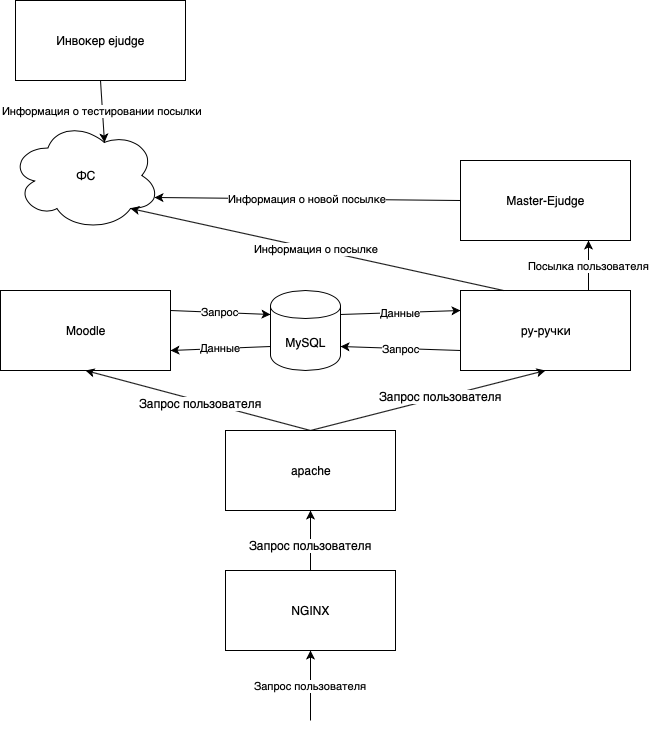
\includegraphics[width=\textwidth]{figures/old_informatics.png}
  \caption{Схема работы Информатикс}
  \label{fig:old_informatics}
\end{figure}

Системы Информатикс развёрнуты на двух раличных виртуальных машинах,
виртулизированных с помощью технологии KVM.

KVM (англ. Kernel-based Virtual Machine) -- программное решение,
обеспечивающее виртуализацию в среде Linux на платформе x86.
Программное обеспечение KVM состоит из загружаемого модуля ядра (называемого kvm.ko),
предоставляющего базовый сервис виртуализации, процессорно-специфического загружаемого модуля kvm-amd.ko либо kvm-intel.ko, 
и компонентов пользовательского режима (модифицированного QEMU). 
Все компоненты программного обеспечения KVM открыты.

На каждой из виртуальных машин развёрнуты разные сервисы:

\begin{itemize}
    \item На первой машине, называемой moodle-vm, развёрнуты сервисы, обслуживающие пользовательский интерфейс -- NGINX, Moodle и py-ручки,
    а так же СУБД MySQL.
    \item На второй машине развёрнуты инстансы Ejudge-системы, Ejudge-Мастер и Ejudge-инвокеры.
\end{itemize}

Схему соотношения сервисов и виртуальных машин можно посмотреть на рисунке \ref{fig:old_vm}.

\begin{figure}
  \centering
  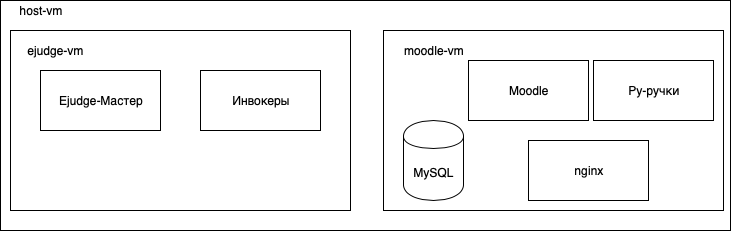
\includegraphics[width=\textwidth]{figures/old_vm.png}
  \caption{Схема виртуальных машин Информатикс}
  \label{fig:old_vm}
\end{figure}

\section{Постановка задачи}

Для решения указанных выше проблем необходимо разработать и улучшить архитектуру, чтобы:

\begin{itemize}
    \item Уменьшить нагрузку на ФС, которой сложно предоставлять доступ к большому количеству файлов.
    \item Добавить возможность встраивать несколько различных тестирующих систем, включая тестирующие системы отличные от Ejudge.
    \item Исправить и ускорить сбор данных для мониторов.
    \item Сократить или полностью избавиться от необходимости использования SQL-запросов, обращающихся к разным БД.
    \item Улучшить общую производительность системы.
    \item Улучшить взаимодействия пользователей с системой 
    -- сделать так, чтобы ошибка отправки решений пропала,
    а посылки принимались сразу и последовательно тестировались.
\end{itemize}

Также необходимо разработать и реализовать архитектурный задел для дальнейшего развития Информатикс в качестве базы задач для встраивания в другие системы.

Помимо этого, нужно разарботать и реализовать план изменения архитектуры системы таким образом, чтобы недоступность системы была минимальной.

\chapter{Программы и алгоритмы, используемые для решения задачи}

Рассмотрим архитектурные изменения, которые были реализованы в рамках решения поставленных задач, 
а так же разберём план изменения архитектуры, позволяющий достигнуть минимальную недоступность системы.

\section{Общие принципы решения}

Было принято решение выделить новый сервис, названный <<Rmatics>>, который должен инкапсулировать в себе работу с посылками, протоколами и тестированием, 
а так же в будущем предоставлять API для тестирования посылок из сторонних систем.

Rmatics -- сервис, предоставляющий API для сдачи задач, обновления их результатов и доступа к протоколам тестирования. 
Помимо этого, Rmatics предоставляет интерфейс для получения данных мониторов.

Rmatics реализован на языке программирования Python и web-фреймворке Flask с использованием SQLAlchemy.

Рассмотрим подробнее причины выбора этих инструментов. Основных причин использовать язык Python -- две:

\begin{enumerate}
    \item Часть функционала уже была написана на Python, при реализации которого были написаны основные модели для БД (на фреймворке SQLAlchemy).
    \item Python позволяет быстро реализовывать необходимый программный код, 
предоставляя высокоуровневые абстракции и огромное количество различных библиотек и программных модулей, заточенных под решение различных задач.
\end{enumerate}

\section{Очередь сдачи посылок}

Для решения проблемы ошибок отправки решений было принято решение использовать очередь (структура данных FIFO).

Рассмотрим некоторые возможности реализации таких очередей с использованием языка программирования Python.

Для Python существует несколько таких систем:

\begin{itemize}
    \item Celery
    \item RQ
    \item 
\end{itemize}{}

В качестве бэкенда для очереди отправки сообщений можно было выбрать следующие технологии:

\begin{itemize}
    \item 
\end{itemize}

Выбор пал на СУБД \texttt{Redis}.

% TODO: ОБЯЗАТЕЛЬНО назвать воркеры rmatics-workers

\section{Идентификаторы посылок}

Для решения проблемы отсутствия уникального идентификатора посылки было принято решение создать новую таблицу с посылками,
в которой доступ к посылок будет реализован с помощью уникального идентификатора -- поля "id". \label{lab:pynformatics_run_id}
Для сохранения однозначности между посылками Ejudge и записями в новой таблице, так же будут сохранены идентификаторы из Ejudge --
номер посылки (поле "ej\_run\_id") и номер контеста "ej\_contest\_id". 
Так же в рамках идеи о возможности использовать как нескольтко различных систем Edjuge, так и других тестирующих систем, 
сохраняется идентификатор текущей тестирующей системы (поле "ejudge\_url").

Для связи посылки с задачей для каждой посылки и для поиска посылок сохранятеся идентификатор задачи ("problem\_id").

Для связи с пользователем сохраняется идентификатор пользователя ("user\_id").

Также сохраняются результаты тестирования -- статус посылки ("ej\_status"), количество пройденных тестов ("ej\_test\_num"), набранный балл ("ej\_score") и другое.

Таким образом, схема таблицы посылок ("pynformatics.run") представляется в следующем виде:

\begin{center}
  \begin{longtable}{|p{0.20\textwidth}|p{0.20\textwidth}|p{0.5\textwidth}|}
    \caption{Схема таблицы pynformatics.run}
    \label{tab:longtable}
    \\ \hline
    Название & Тип данных & Комментарий \\
    \hline \endfirsthead
    \subcaption{Продолжение таблицы~\ref{tab:longtable}}
    \\ \hline \endhead
    \hline \subcaption{Продолжение на след. стр.}
    \endfoot
    \hline \endlastfoot
    id              & INTEGER     & Идентификатор посылки \\
    \hline
    ej\_run\_id     & INTEGER     & Номер посылки в ejudge \\
    \hline
    ej\_contest\_id & INTEGER     & Номер контеста в ejudge \\
    \hline
    ejudge\_url     & INTEGER     & Идентификатор тестирующей системы \\
    \hline
    user\_id        & INTEGER     & Идентификатор пользователя \\
    \hline
    problem\_id     & INTEGER     & Идентификатор задачи \\
    \hline
    ej\_status      & INTEGER     & Статус тестирования \\
    \hline
    ej\_test\_num   & INTEGER     & Количество пройденных тестов \\
    \hline
    ej\_score       & INTEGER     & Набранный балл \\
    \hline
  \end{longtable}
\end{center}

Однако при подходе с новой таблицей посылок появилась следующая проблема:
ejudge всё ещё пишет данные о результатах системы в свои таблицы БД ejudge
и не позволяет тривиально узнать о том, что посылка протестирована (подробнее рассмотрено в пункте \ref{chap:inotify}).

Решить эту проблему можно двумя способами:

\begin{itemize}
    \item создать специальный триггер в БД, который будет срабатывать при изменении результата тестирования;
    \item создать сервис, ждущий информации об обновлении посылки и каким-либо образом заставить ejudge отправлять сообщение при изменении статуса посылки, в таком случае сервис должен быть асинхронным, так как ejudge -- синхронен, и, если обновление посылки затянется, ejudge будет простаивать.
\end{itemize}

Рассмотрим подробнее оба способа.

\begin{center}
  \begin{longtable}{|p{0.40\textwidth}|p{0.20\textwidth}|p{0.30\textwidth}|}
    \caption{Способы решения проблемы обновления статусов в pynformatics.runs}
    \label{tab:longtable}
    \\ \hline
    Критерий & Триггер в БД & Сервис, ждущий обновления посылок \\
    \hline \endfirsthead
    \subcaption{Продолжение таблицы~\ref{tab:longtable}}
    \\ \hline \endhead
    \hline \subcaption{Продолжение на след. стр.}
    \endfoot
    \hline \endlastfoot
    Снижение производительности & Значительное & Незначительное \\
    \hline
    Сложность реализации    & Просто     & Сложно \\
    \hline
    Сложность поддержки & Просто     & Сложно \\
    \hline
  \end{longtable}
\end{center}

Был проведён эксперимент, реализующий подход с триггером, производительность БД упала очень значительно, поэтому финальным вариантом был выбран отдельный асинхронный сервис, ждущий информацию посылки посылки.

\subsection{Сервис, ждущий обновление посылки}

\label{lab:ejudge_listener}
Для начала, необходимо было понять, что нужно сделать, 
чтобы ejudge смог отправлять сообщение об обновлении посылки.
Было решено изменить код обновления статуса посылки таким образом, 
чтобы тот после обновления статуса тестирования БД исполнял дополнительный код,
оповещающий об изменении посылки. В листинге \ref{lst:ejudge_http_notify} представлен код, оповещающий об обновлении посылки.

Затем необходимо было выбрать протокол общения между ejudge и сервисом.
Для упрощения реализации вызываемого кода был выбран протокол HTTP.

Сервис, ждущий обновление посылки, был назван ejudge-listener.

\lstinputlisting[language=C,caption={Код, оповещающий об обновлении посылки},label=lst:ejudge_http_notify]{listings/ejudge_http_notify.c}

Код ejudge-listener был реализован с помощью языка программирования Python.
Для того, чтобы сделать ejudge-listener асинхронным, можно было выбрать один из следующих способов: 

% Celery vs RQ vs Асинхронщина

Так как обновление статуса посылки является критически важным функционалом системы,
и терять эту информацию -- недопустимо, было принято решение использовать фреймворк Celery.

Для инкапсуляции логики работы с таблицей pynformatics.run, 
доступ к ней есть только у сервиса Rmatics, 
поэтому ejudge-listener не обновляет данные этой таблицы самостоятельно,
вместо этого он передаёт по протоколу HTTP запрос на изменение посылки в Rmatics.

Полная схема работы ejudge-listeenr представлена на Рис. \ref{fig:ejudge_listener}.



\section{Хранение посылок и результатов тестирования}

Необходимо было разработать способ уменьшить нагрузку на ФС.
На файловой системе хранился код посылок пользователей,
протоколы и результаты тестирования.
Можно выделить следующие кейсы, нагружающие ФС (все кейсы значительно нагружают ФС из-за наличия десятков миллионов маленьких файлов, делая доступ к файлу медленным):

\begin{enumerate}
    \item Оправка посылки -- Master-ejudge сохраняет отправленные посылки в ФС для дальнейшего их тестирования Инвокерами.
    \item Сохранения протоколов и результатов тестирования -- Инвокеры после тестирования посылки отправляют сохраняют их на ФС.
    \item Просмотр посылки -- при просмотре исходного кода пользователем py-ручки берут его из ФС.
    \item Просмотр протокола и результатов тестирования -- при просмотре протокола и результатов тестирования py-ручки берут их из ФС.
    \item Бэкапы данных о посылках и протоколах.
\end{enumerate}

Так вносить изменения в работу ejudge -- дорого и нетривиально, 
нагрузка, даваемая пунктами а и б может быть уменьшена единственным способом:
уменьшением количества сохранённых таким образом на ФС файлов.

Для того, чтобы удалить файлы из ФС, 
не потеряв при этом исходники посылок пользователей и их протоколы, 
необходимо предварительно сохранить файлы из ФС в другое хранилище.
Это хранилище может быть реализовано с помощью одной из существующих СУБД.
В таком случае, маленькие файлы могут храниться внутри больших блобов (англ. Binary Large Object — двоичный большой объект).

Проблемы в и г также решаются введением нового хранилища:
результаты тестирования и посылки, запрашиваемые пользователями будут доставаться из нового хранилища.

Скорость доступа к ним может быть в таком случае увеличена с использованием индексов.

В качестве ключа индекса будет использован идентификатор посылки новой таблицы pynfornatics.runs, id (подробнее описано в главе \ref{lab:pynformatics_run_id}).

Проблему с бэкапами можно решить следующим способом:
во-первых, нагрузка на ФС и так уменьшится из-за бэкапа блобов, а не маленьких файлов, 
во-вторых, если выбранная СУБД будет иметь возможность создания реплик, 
можно будет создать одну из таких реплик на другом сервере, синхронизируя её с основным экземпляром через сеть Интернет, и делать бекапы на нём. 
В таком случае, нагрузка на ФС основного сервера при проведении бекапов расти не будет.

Необходимо отметить, что протоколы тестирования по своей структуре -- 
плохо структурированные небольшие файлы, которые можно представить в виде набора JSON-ов.
В качестве хранилища для исходников и протоколов была выбрана СУБД MongoDB, так как она хорошо подохдит дляхранения плохо структурированных данных\cite{mongo_good_for_unstruct}.

MongoDB (от англ. humongous — огромный) -- документоориентированная СУБД с открытым исходным кодом, не требующая описания схемы таблиц. 
MongoDB классифицирована как NoSQL, и использует JSON-подобные документы и схему базы данных. 
MongoDB (с дефолтным движком WiredTiger\cite{mongo_store_engine}) хранит данные в блобах\cite{mongo_wiredtiger}, поддерживает индексирование и имеет функционал репликации\cite{mongo_indexes}\cite{mongo_replicas}.

Для хранения данных в MongoDB были использованы следующие схемы:

\begin{itemize}
    \item protocol -- для хранения протоколов и результатов тестирования;
    \item source -- для хранения исходного кода пользователей.
\end{itemize}

Сохранить существующие данные с ФС в MongoDB -- тривиально,
но что делать с новыми протестированными посылками?
В новой архитектуре Информатикс уже есть сервис, 
который знает, что посылка протестировалась -- это ejudge-listener (подробнее описан в главе \ref{lab:ejudge_listener}).

Для сохранения новых протестированных посылок, 
функциональность сервиса ejudge-listener была расширена 
-- при получении обновлении посылки ejudge-listener теперь забирает протокол посылки и результат тестирования из ФС и сохраняет в MongoDB.

\begin{figure}
  \centering
  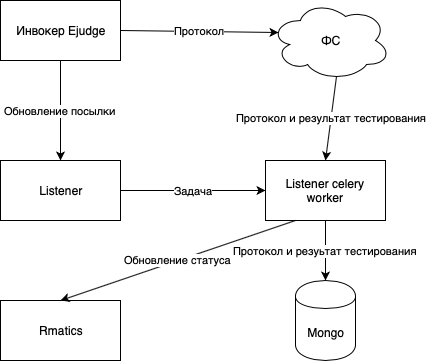
\includegraphics[width=\textwidth]{figures/listener.png}
  \caption{Схема работы ejudje-listener}
  \label{fig:ejudge_listener}
\end{figure}




\section{Мониторы}

Мониторы -- результаты прохождения группой учеников наборов контестов.
Они предоставляют информацию о том, решена ли задача в контесте,
и сколько было неудачных попыток решения или итоговый балл. 
Примеры мониторов представлены на Рис. \ref{fig:monitor_acm} и Рис. \ref{fig:monitor_ioi}.
Сбор результатов прохождения контестов был очень ресурсоёмкой задачей,
которая сильно нагружала Информатикс.

\begin{figure}
  \centering
  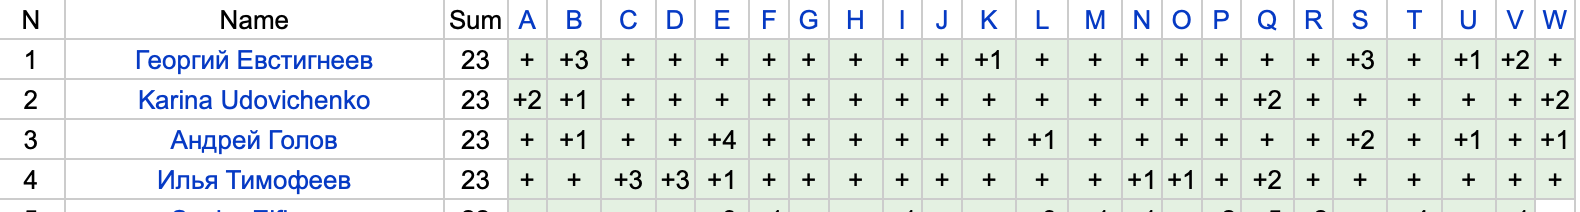
\includegraphics[width=\textwidth]{figures/monitor_acm.png}
  \caption{Монитор Информатикс для типа соревнования типа ACM}
  \label{fig:monitor_acm}
\end{figure}

\begin{figure}
  \centering
  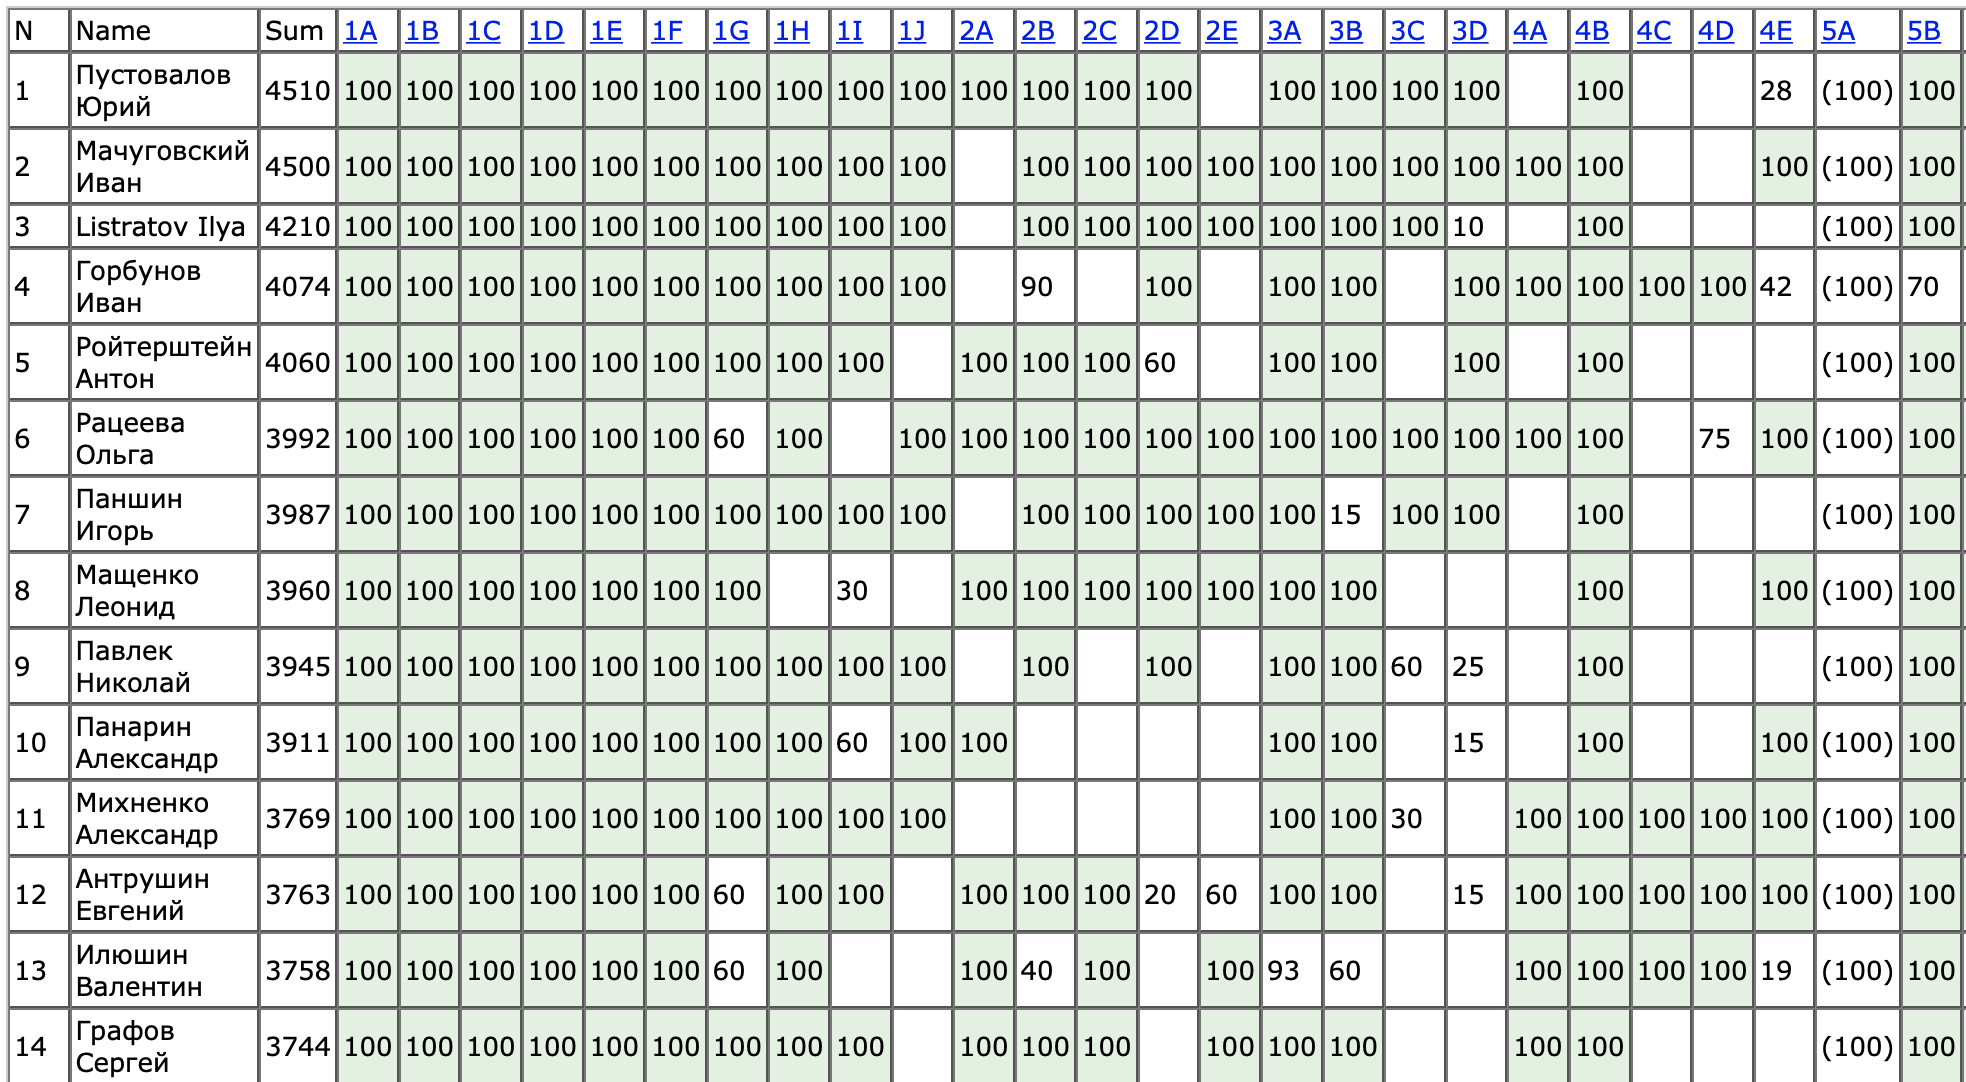
\includegraphics[width=\textwidth]{figures/monitor_ioi.png}
  \caption{Монитор Информатикс для типа соревнования типа IOI}
  \label{fig:monitor_ioi}
\end{figure}

Один сбор результатов о тестировании через новую таблицу (см. Главу \ref{lab:pynformatics_run_id}) может занимать в зависимости от общей нагрузки на БД до десятков минут, что неприемлимо.

Для того, чтобы ускорить отображение результатов прохождения учениками контестов, 
а так же уменьшить нагрузку, которую даёт сбор результатов, 
было принято решение использовать кэширующую систему\cite{cache_abstract}.

\subsection{Инвалидация кэша}

Кэширующие системы могут использовать различные приёмы для того, чтобы очищать кэш, когда он перестаёт быть валидным.
% TODO: из чего состоит кэш
Один из таких методов -- время жизни (англ. TTL -- Time To Live).
Этот метод прост в реализации, однако
при его использовании возникает проблема -- 
часть данных, отдаваемых пользователю, становится неликвидными.
Более того, чем дольше время жизни кэша, тем больше неликвидных данных получает пользователь.

Другой из методов -- очищать необходимый кэш если в системе происходят какие-либо события, изменяющие исходные данные.
Такой метод называется инвалидацией кэша.

Использовать метод, основанный только на времени жизни для результатов пользователей неверно, 
так как результаты меняются часто, и пользователям сразу важно видеть,
какое место в итоговой таблице они занимают.

Было принято использовать комбинированный метод кэширования, 
основанный как на времени жизни, так и на инвалидации кэша.

Время жизни эмпирическим путём было выбрано в одни сутки.

Код, реализующий сбор данных для монитора был реализован в системе Rmatics и представлен на листинге \ref{lst:getruns}. 
Данный код формирует данные по мониторам и возвращает их в формате JSON.

\lstinputlisting[language=Python,caption={Код, реализующий сбор данных для монитора.},label=lst:getruns]{listings/get_monitors.py}

Для инвалидации кэша результатов тестирования важно понимать, 
какие именно действия в системе приводят к изменению изначальных данных.
Эти действия -- изменения статуса посылки.
Статус посылки в БД меняется в двух случаях -- после тестирования посылки (см Рис. \ref{lab:ejudge_listener}) и при изменении статуса посылки пользователем через Web-интерфейс. 
Важно помнить, что при обновлении посылки из ejudge-listener нельзя, не используя дополнительных запросов,
получить ни идентификатор контеста, в рамках которого отправлено решение, 
ни идентификатор групп, в которых состоит пользователь, отправивший посылку.
В то же время, на этом этапе доступен идентификатор задачи и идентификатор пользователя.
Также стоит отметить, что оба действия инкапсулированы в сервис Rmatics.

Также для реализации кэша важно понимать, 
как правильно разделить кэшируемые данные.

В запросе на результаты тестирования от пользователей фигурируют следующие данные: 

\begin{itemize}
    \item Идентификатор группы пользователей.
    \item Идентификатор контеста или набор идентификаторов контестов.
    \item Ограничение по временному отрезку, в котором учитываются посылки.
\end{itemize}

Можно было бы использовать эти идентификаторы для создания ключей кэшей,
однако в таком случае каждая новая посылка любого пользователя из группы в один из контестов заставляла бы систему инвалидировать кэш,
что вело бы к постоянным повторным сборам кэшей.

Поэтому было принято разбить кэш результатов контестов на более мелкие части -- по одной на каждую задачу контеста.
В таком случае, длительность жизни каждого кэша увеличивалась,
а количество кэшей, которые нужно инвалидировать при отправке пользователем посылки -- уменьшалась.

Для того, чтобы не делать при инвалидации кэша дополнительных запросов в БД,
было решено использовать в качестве ключа кэширования не идентификатор группы,
но идентификаторы пользователей в этой группе.

\subsection{Хранение кэша}

Система, в которой хранится кэш, должна обладать следующими характеристиками:

\begin{itemize}
    \item иметь потенциальную возможность встроить инвалидацию кэша;
    \item быть удобно приспосабливаемой под задачи хранения данных типа ключ-значение;
    \item быть быстрой как для операций сохранения кэша, так и для операций выдачи данных;
    \item быть удобной в эксплуатации;
    \item желательно, чтобы система могла уметь инвалидировать значения по времени.
\end{itemize}

Рассмотрим несколько возможных вариантов для хранилища кэша.
Так как в Информатикс уже и так достаточное количество различных специфичных хранилищ, 
будем рассматривать только уже используемые на сайте системы.

Стоит сразу отбросить web-сервер nginx, так как,
хоть он и предоставляет возможность кэшировать данные,
нет никакой тривиальной возможности тривиально инвалидировать кэш после изменения статуса посылки.

Таким образом, под сравнение попадают MySQL, MongoDB и Redis. Рассмотрим так же возможность реализовать кэш на файловой системе.

\begin{center}
  \begin{longtable}{|c|c|c|c|p{0.20\textwidth}|}
    \caption{Сравнение систем для хранения кэша}
    \label{tab:cache_systems}
    \\ \hline
    Название & Ключ-значение & Скорость & Удобство & Инвалидация по времени \\
    \hline \endfirsthead
    \subcaption{Продолжение таблицы~\ref{tab:longtable}}
    \\ \hline \endhead
    \hline \subcaption{Продолжение на след. стр.}
    \endfoot
    \hline \endlastfoot
    Redis  & Да & Очень быстро & Очень удобно & Есть \\
    \hline
    MySQL  & Реализуемо & Быстро & Удобно & Нет \\
    \hline
    MongoDB  & Да & Быстро & Удобно & Нет \\
    \hline
    ФС  & Да & Медленно & Не удобно & Нет \\
    \hline
  \end{longtable}
\end{center}

По совокупности причин, приведённых выше, 
а так же по результатам сравнения в Таблице \ref{tab:cache_systems},
в качестве системы хранения кэша была выбрана СУБД Redis.

Для быстрого поиска кэша по ключу в Redis, 
было решено ограничить длину ключа, взяв MD5 хэш от аргументов запроса на выдачу данных монитора. 
MD5-хэш был создан для того, чтобы создавать компандиум (англ. message digest) для входного сообщения\cite{md5}.
Код, который используется для создания хэша от аргументов запроса представлен на листинге \ref{lst:md5}.

\lstinputlisting[language=Python,caption={Код создания хэша от аргументов запроса.},label=lst:md5]{listings/make_md5.py}

\subsection{Хранение данных для инвалидации кэша}

Для того, чтобы при обновлении статуса посылки, 
инвалидировались только нужные ключи, 
необходимо сохранить связь, между аргументами, по которым собирались данные,
в случае мониторов это идентификаторы пользователей и идентификаторы задач, 
и хэшами, эти данные хранящими.

Для этого было решено сохранять эту информацию о хэшах в СУБД MySQL.
Принимая во внимание то, что аргументы могут быть различны,
а их количество может меняться,
информацию предполагалось хранить в таблице "monitor\_cache\_meta".
Таблица должна была иметь два поля -- invalidate\_args и key.
В поле invalidate\_args должны были храниться данные об аргументах, 
с помощью которых был создан кэш, 
а в поле key должен был храниться ключ из Redis, 
по которому кэш был доступен. 

Для поля invalidate\_args ыла разработана следующая спецификация: 
аргументы, по которым собирались данные, отображались в строки, 
где сначала шло название аргумента, затем аргумент, 
и затем разделитель между аргументами.

Например, если приходили следующие аргументы, пользователь=1, пользователь=2, задача=3, а разделителем был задан символ <<|>>, то результирующей строкой было бы \textit{пользователь=1|пользователь=2|задача=3}.

В таком случае, если новая посылка пользователя 1 по задаче 3 протестировалась бы, можно было бы найти этот кэш запросом в БД,
с использованием полнотекстового поиска, например, следующим SQL-запросом:

\lstinputlisting[language=SQL,caption={Код создания хэша от аргументов запроса.},label=lst:md5]{listings/select_cache_meta.sql}

С таблицей, сохраняющей аргументы, с которыми был создан кэш,
и ключами хэшей, появилась новая проблема:
при каждой перегенерации кэша создалась запись в БД, и размер таблицы постоянно рос.
Было принято решение добавить поле "when\_expire", которое бы хранило время, когда кэш устаревал, и настроить скрипт автоматического удаления строк из БД,

Такая реализация максимально гибка; её можно использовать не только для таблиц результатов,
но и для каких-либо требующих инвалидации кэшей в будущем.

Однако, эта реализация нагружала БД, так как для инвалидации постоянно требовалось сканировать все строки "invalidate\_args"
, что доволно медленно.
Такая нагрузка была неприемлимой.
Поэтому было принято решение добавить в таблицу идентификатор задачи, "problem\_id".

Итоговая схема таблицы представлена в таблице \ref{tab:cache_meta}.

\begin{center}
  \begin{longtable}{|p{0.20\textwidth}|p{0.20\textwidth}|p{0.5\textwidth}|}
    \caption{Схема таблицы pynformatics.run}
    \label{tab:cache_meta}
    \\ \hline
    Название & Тип данных & Комментарий \\
    \hline \endfirsthead
    \subcaption{Продолжение таблицы~\ref{tab:cache_meta}}
    \\ \hline \endhead
    \hline \subcaption{Продолжение на след. стр.}
    \endfoot
    \hline \endlastfoot
    id              & INTEGER     & Идентификатор записи \\
    \hline
    key     & CAHR(128)     & Ключ в Redis \\
    \hline
    problem\_id     & INTEGER     & Идентификатор задачи \\
    \hline
    invalidate\_arg & TEXT     & Аргументы для инвалидации \\
    \hline
    when\_expire     & DATETIME     & Время, когда кэш станет невалидным \\
    \hline
  \end{longtable}
\end{center}

\subsection{Защита от гонки данных}

Существуют ситуации, в которых множество пользователей одновременно запрашивают данные результатов одного и того же соревнования.
В таких случаях происходит следующее:

\begin{enumerate}
    \item Приходит запрос на формирование данных от пользователя №1.
    \item В кэше данных ещё нет, значит, данные нужно собрать.
    \item Данные для пользователя №1 начинают собираться. 
    Как было отмечено выше, процесс сбора данных может занимать значительное время.
    \item Приходит запрос на формирование данных от пользователя №2.
    \item Данные для пользователя №1 собраны и положены в кэш.
    \item Пользователь №1 получает данные.
    \item Данные для пользователя №2 начинают собираться.
    \item Данные для пользователя №2 собраны и положены в кэш.
    Это ровно те же данные с ровно таким же ключом кэша, которые были сохранены во время обработки запроса от пользователя №1.
    \item Пользователь №2 получает данные.
\end{enumerate}

Такой порядок выполнения действий заставляет систему несколько раз собирать одни и те же данные вместо того, чтобы взять их из кэша. Более того, стоит отметить, что пользователь №2 мог получить данные гораздо позже пользователя №1, так как шаги в и ж могут выполняться долго.

Такая проблема так же может называться гонкой данных (англ. race condition)\cite{race_condition}.

Необходимо было сделать так, чтобы не смотря на то, 
что множество пользователей одновременно запрашивают данные результатов одного и того же соревнования, 
данные собирались только один раз (конечно, учитывая то, что в это время кэш может инвалидироваться).

Для этого было решено реализовать мьютекс, который блокировал бы сбор данных по определённому ключу.

Мьютекс (англ. mutex, от mutual exclusion -- <<взаимное исключение>>) -- аналог одноместного семафора, служащий для синхронизации одновременно выполняющихся потоков. 
Мьютекс отличается от семафора тем, что только владеющий им поток может его освободить, т.е. перевести в отмеченное состояние. 
В данном случае под потоками понимаются потоки выполнения запросов на сбор мониторов.

Для того, чтобы мьютекс можно было эффективно и удобно использовать в различных инстансах сервиса Rmatics, 
было решено реализовать его при помощи СУБД Redis. 
СУБД Redis имеет необходимые характеристики для того, 
чтобы эффективно реализовать мьютекс\cite{carlson2013redis}.
В качестве алгоритма был выбран алгоритм <<Redlock>>\cite{redis_lock_base}.
Этот алгоритм предоставляет возможность безопасно реализовывать блокирующие системы на кластере из СУБД Redis\cite{redis_lock_answer}.

В качестве реализации <<Redlock>> была использована библиотека <<Redlock-py>>.
Для работы системы был реализован прикладной код, реализующий логику, представленную в листинге Алгоритм \ref{alg:lock}. 

\begin{rualgorithm}[H]
 \KwData{Ключ хэша}
 \KwResult{Поток захватит мьютекс}
 инициализация\;
 Мьютекс = не захваченный Мьютекс\;
 \While{Мьютекс не захвачен}{
    Мьютекс = попытаться захватить с ключом хэша\;

  \eIf{Мьютекс не захвачен}{
  спать 0,4 секунды\;
   }{
     выйти из цикла\;
  }
 }
 \caption{Алгоритм захвата мьютекса}
 \label{alg:lock}
\end{rualgorithm}

В результате работы этого алгоритма, поток, обрабатывающий пользователя №2,
получит данные из кэша, 
и не позднее, чем через 0,4 секунды после потока (опуская время доступа к кэшу и то, что планировщик ОС может выделить время для работы потока несколько позже), обрабатывающего запрос пользователя №1.

\subsection{Выводы по подразделу}

В данной главе была рассмотрена проблема формирования данных о результатах пользователей.
Были разработаны и реализованы:

\begin{itemize}
    \item механизм кэширования данных;
    \item механизм инвалидации кэшей;
    \item механизм предотвращения гонок данных.
\end{itemize}

Иллюстрация, демонстрирующая схему работы запроса мониторов представлена на рисунке \ref{fig:cache_system}.

\begin{figure}
  \centering
  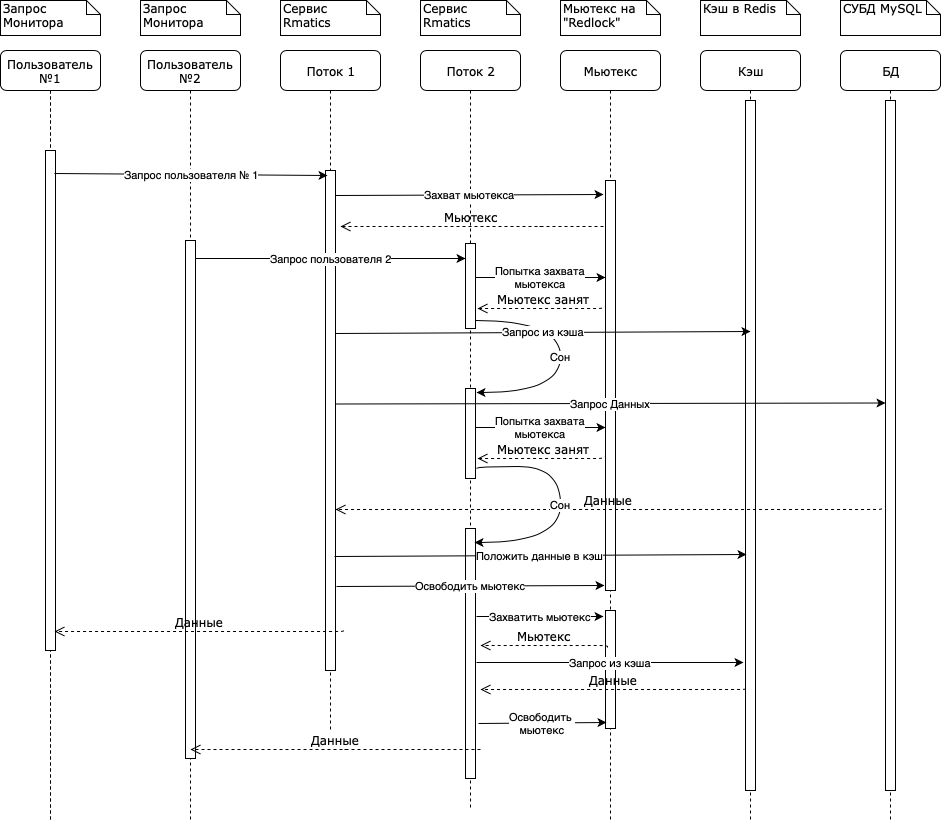
\includegraphics[width=\textwidth]{figures/cache_system.png}
  \caption{Временная диаграмма запроса мониторов двумя пользователями}
  \label{fig:cache_system}
\end{figure}


\section{План изменения архитектуры}

План изменения архитектуры должен представлять собой 
последовательные шаги для внедрения новой архитектуры в старую систему.

Важно понимать, что сложно внедрить всю архитектуру целиком, и лучше использовать для этого отдельные шаги.

Помимо этого, отдельные шаги позволяют так же протестировать различные системы и приобрести уверенность, 
что итоговая реализация архитектура будет корректно работать и успешно справляться с необходимыми нагрузками.

План переноса архитектуры можно разделить на четыре основные части:

\begin{itemize}
    \item Разворачивание основных систем.
    \item Перенос данных в новые схемы и хранилища.
    \item Пошаговая замена и встраивание различных сервисов в текущую систему.
    \item Полный переход на новую архитектуру.
\end{itemize}

\subsection{Разворачивание основных систем}

Предварительно необходимо развернуть необходимые системы, такие как:

\begin{itemize}
    \item СУБД MongoDB для хранения исходных кодов пользователя и протоколов тестирования.
    \item СУБД Redis для хранения кэшей и в качестве бэкенда для воркеров ejudge-listener и Rmatics.
    \item Rmatics в качестве основной системы;
    \item ejudge-listener для обновления статусов посылок и сбора протоколов;
\end{itemize}

Для разворачивания СУБД MongoDB в CentOS достаточно добавить официальный репозиторий MongoDB и установить необходимый пакет через стандартный менеджер пакетов yum.

Однако опытным путём было выяснено, что стандартный конфигурационный файл
обладал существенным недостатком: он не ограничивал количество потребляемой кэшом СУБД оперативной памяти (оперативное запоминающее устройство, ОЗУ).
Данный недостаток был исправлен добавлением в конфигурационный файл максимального количества потребляемой кэшами СУБД.

MongoDB будет запускаться и управляться стандартным для CentOS способом,
с помощью системы systemd.
Конфигурационный файл systemd (юнит) был автоматически добавлен при установке.

Для разворачивания СУБД Redis нужно установить пакет Extra Packages for Enterprise Linux (EPEL) \cite{redis_install}.
Затем можно будет установить СУБД Redis через стандартный менеджер пакетов yum.

Redis будет запускаться и управляться стандартным для CentOS способом,
с помощью системы systemd.
Конфигурационный файл systemd (юнит) был автоматически добавлен при установке.

Установка реализованных сервисов, таких как ejudge-listener и Rmatics потребудет больше усилий.

Оба сервиса написаны на Python и требуют установки различных Python-пакетов для корректной работы.
Для установки различных окружений был использован стандартный для Python менеджер пакетов -- pip и утилита для управлений окружениями Python virtualenv. Оба сервиса будут работать под управлением стандартной для CentOS системы systemd.

Для удобной установки и дальнейшего обновления сервисов были написаны конфигурационные файлы (роли) с помощью использования технологии Ansible.

Ansible -- система управления конфигурациями, написанная на Python, с использованием декларативного языка разметки для описания конфигураций.
Используется для автоматизации настройки и развертывания программного обеспечения. 
Обычно используется для управления Linux-узлами, но Windows также поддерживается. 
Поддерживает работу с сетевыми устройствами, на которых установлен Python версии 2.4 и выше по SSH или WinRM соединению.

Ansible-роли совершают следующие действия для установки сервисов на целевых серверах:

\begin{itemize}
    \item архивируют исходный код;
    \item доставляют исходный код на сервер;
    \item создают необходимые Python-окружения при помощи virtualenv;
    \item перемещают исходный код в необходимые директории;
    \item при необходимости обновляют необходимые systemd-юниты;
    \item запускают или перезапускают сервисы.
\end{itemize}

\subsection{Перенос данных в новые системы и хранилища}

\label{chap:move_data}
Для того, чтобы новая система начала функционировать,
необходимо было осуществить перенос данных из текущих хранилищ в новые.

Нужно скопировать информацию о посылках из текущих таблиц в таблицу pynfotmatics.runs. 
Также нужно перенести данные с файловой системы в СУБД MongoDB.

Для того, чтобы скопировать информацию о посылках из текущих таблиц, 
был написан скрипт на языке SQL, копирующий данные в pynformatics.runs.

Чтобы не нагружать Информатикс, был создан бэкап СУБД MySQL,
который затем был развёрнут на другом сервере. 
Был запущен SQL-скрипт, и таблица pynformatics.runs наполнилась необходимыми данными.
После этого был создан бэкап отдельной таблицы, pynformatics.runs.
Этот бэкап был перенесён на основной сервер Информатикс, а затем был запущен механизм восстановления данных в нужную таблицу.

Таким образом было перенесено более 15 миллионов посылок.
Однако стоит учесть, что посылки, которые появлялись начиная со времени бэкапа СУБД MySQL из Информатикс и до введения отправки посылок через Rmatics,
в pynformatics.runs не перенесены, и был написан отдельный SQL-скрипт,
добавляющий в pynformatics.runs только недостающие посылки.

Для того, чтобы перенести данные о результатах тестирования и исходных кодах пользователя, 
были предприняты аналогичные действия.

Чтобы не нагружать сайт, бэкап посылок и протоколов был развёрнут на другом сервере.
Был написан скрипт на Python, собирающий протоколы и исходный код, 
и сохраняющий данные в MongoDB. 

После этого СУБД MongoDB на этом сервере была остановлена, 
а блобы базы данных были перенесены на сервер Информатикс.
Затем эти блобы были перенесены в директорию данными MongoDB.

Таким образом было перенесено более 15 миллионов исходных кодов, протоколов и результатов тестирования.
Однако стоит учесть, что данные, которые появлялись начиная со времени бэкапа ФС из Информатикс и до введения отправки посылок через Rmatics,
в MongoDB не перенесены, и был написан отдельный Python-скрипт,
переносящий в MongoDB только недостающие исходные коды, протоколы и результаты тестирования.

\subsection{Пошаговое встраивание сервисов}

Для того, чтобы аккуратно совершить переход на новую архитектуру, 
а так же протестировать различные системы и приобрести уверенность в разработанных решениях, было принято вводить функциональность сервисов постепенно.

Был отмечен важный для такого подхода факт факт: 
сервер тестирования Ejudge готов был обработать двукратное увеличение посылок от пользователей.

Как было рассмотрено в главе \ref{chap:move_data}, 
данные после первичного переноса из бэкапов, начали рассинхронизироваться с актуальной информацией о посылках.

Поэтому было принято решение дублировать отправку посылок: 
py-ручки были изменены таким образом, чтобы при отправке посылки в Ejudge,
послыка также отправлялась бы и в Rmatics.
Rmatics затем так же пересылал эту посылку в Ejudge, 
Очевидно, что идентичные 

Это дало возможность сразу решить проблему рассинхронизации от рассинхронизи


\backmatter %% Здесь заканчивается нумерованная часть документа и начинаются ссылки и
            %% заключение

\chapter{Заключение}

В работе использовалась система сиамских нейронных сетей, однако, в перспективе, будет возможно использовать динамическую маршрутизацию между нейронами для уменьшения ошибок распознавания объектов, например, в случаях, когда пользователь расположил смартфон «вверх ногами».
Описанная система подходит для случаев, когда число пользователей невелико, например, для "мобильного девайса", когда число пользователей ограничено (например, в IPhone, максимальное число отпечатков - 10 для touch id или 2 для face id). 
Метод применим для распознавания подписи человека и в перспективе возможно его использование в программном обеспечении для авторизации пользователя.

\bibliographystyle{gost780u}
\bibliography{main.bib}

%%% Local Variables: 
%%% mode: latex
%%% TeX-master: "rpz"
%%% End: 

\end{document}
